\chapter{Introduction}
% -  What is provenance (stress the more general notion, not just the form used in relational database literature), and why it is useful in managing data 
% -  some tasks users would do with provenance           
% -  quick intro to the PROV standard 
% -  the difficulty handling large PROV collections 
% -  intro to clustering as an approach to reduce clutter of PROV information

% Historically provenance is a record of ownership of a word of art of antique, used as a guide to authenticity or quality. It is also has some use in the field of accounting in relation to auditing and identifying lineage. 

The concept of provenance (from the latin \textit{provenio}, ``to
come forth''), has been around for a long time~\cite{Bearman1985}.
It has been used in many other fields outside of computer science,
primarily that of art and antiques, where the provenance of a piece
is used as a guide to authenticity and quality. It has also been
used in the field of accounting in relation to auditing as well as
in databases, linking tuples in a query output to the reasons they
exist.

In this paper, provenance is a form of metadata representing the
lineage of a dataset or digital object. This is similar to the
information stored in a version control system but
goes beyond versions and authorship 
to capture a wider range of lineage data. 
Provenance makes it possible to identify and trace what other pieces
of information and activities have led to a digital object being in its
current state.

Large amounts of system-level, \textit{observational} provenance can be captured automatically and inexpensively, as in PASS~\cite{Macko2011,180755}. 
User-level provenance, however, depends more on the specific application,
as in Burrito~\cite{Guo2012}, an application created to help automate the more tedious aspects of experiment organisation and note taking. It captures the user activities such as web history, command line arguments and modified files, whilst allowing the user to annotate and view these activities at any time. The captured provenance then supports exploration of a single element. The user can view the provenance of an outputted provenance graph to see versions of the graph as well as the commands and input files used to create it. This allowed users to freely experiment, tweaking arguments and input to create different graphs, knowing that, at any point, they could explore the provenance to find what created any versions of a graph.

Burrito, and similar early interfaces, stored provenance information in a variety flat file formats. Since 2013, the PROV specification~\cite{primer2013} provides a standard generic model for provenance, with well-defined domain-specific extension points and a number of serialisations (RDF, XML, JSON, PROV-N).
%
PROV statements express ``\emph{descriptions of the entities and activities involved in producing and delivering or otherwise influencing a given object}'' and they are underpinned by three main concepts illustrated in Fig.~\ref{fig:key-concepts}:
(i) Entities: Physical, digital, conceptual objects, (ii) Activities: An element that causes an entity to come into existence, and (iii) Agents: Someone or something that can be assigned responsibility for an activity taking place.

\begin{figure}[h]
	\centering
	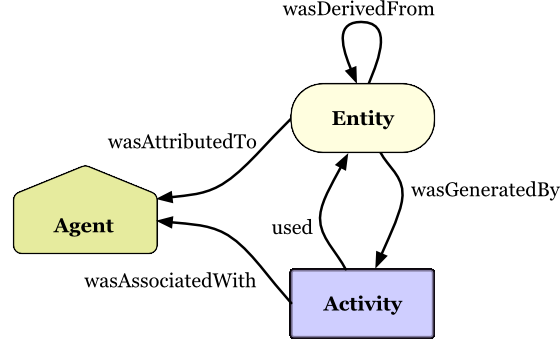
\includegraphics[width=0.4\linewidth]{key-concepts}
	\caption{Key Concepts and relationships from the PROV standard displayed in a labelled acyclic graph.}
	\label{fig:key-concepts}
\end{figure}

Provenance data, especially of the observational, low-level kind, quickly grows in size. Whilst the examples in this paper only show graphs with a small number of nodes, a provenance file can readily grow to millions of nodes. Because provenance stores historical data without summarisation, its grows monotonically over time. The speed of this increase is directly related to the granularity that the captured provenance. So, for example, capturing user actions typically makes the increase slower than is the case for operating system actions. In both cases, however, handling these large graphs causes both technical and usability issues. 

From a technical stand point it becomes resource intensive to scan a provenance file and display a visualisation of it, more so if the application reading the file runs analysis or summarisation of the data. 
%
Even more critically, from a usability perspective, it quickly becomes difficult for a user to interpret and explore such a large amount of information. The question then becomes how to ensure 
%% it is far more than cognitive load so I have altered this -- we can discuss it
%% the cognitive load on 
users can readily understand, explore and find the information they want from a graph. 
We build on research in both provenance~\cite{Seltzer2011, Borkin2013} 
and large scale graphs~\cite{Schaffer1996, Abello2006} 
to tackle this problem by simplifying graphs.
We describe our approach as \emph{clustering}, meaning that we combine multiple nodes into a single node.
This means that there are fewer nodes on the screen, with new combination concepts.

Notable amongst prior attempts at adaptive visualization of provenance graphs is the MapOrbiter~\cite{Macko2011a}, which is based on \textit{semantic zoom} and applies primarily to low-level system provenance, like PASS~\cite{Macko2011}.  One limitation of the approach is that the \textit{semantic} aspect assumes a priori knowledge of the type of processes that appear in the provenance trace,  and of their hierarchical relationships.

Figures~\ref{fig:fitness-ungrouped} and~\ref{fig:fitness-grouped} illustrate our approach
for an entity \texttt{Report}, written by \texttt{Bob}, using information he \texttt{analysed}  based on a \texttt{Fitness-Summary} that was generated by a \texttt{Summarize} script that joins information 
from his own fitness feeds, \{\texttt{Fitbit}, \texttt{GoogleFit}, \texttt{CalorieTracker}\}.
Figure~\ref{fig:fitness-grouped} shows the same provenance graph as Fig.~\ref{fig:fitness-ungrouped} 
after all the nodes related to fitness analysis and summarisation have been clustered into one node \texttt{Fitness Data}. Note the common concepts in these figures: \textit{Bob has written a report regarding fitness data he has analysed himself}. Even this small example illustrates clustering can simplify a graph,
potentially making it more useful if the level of abstraction is right for Bob's needs.

\begin{figure}[h]
	\centering
	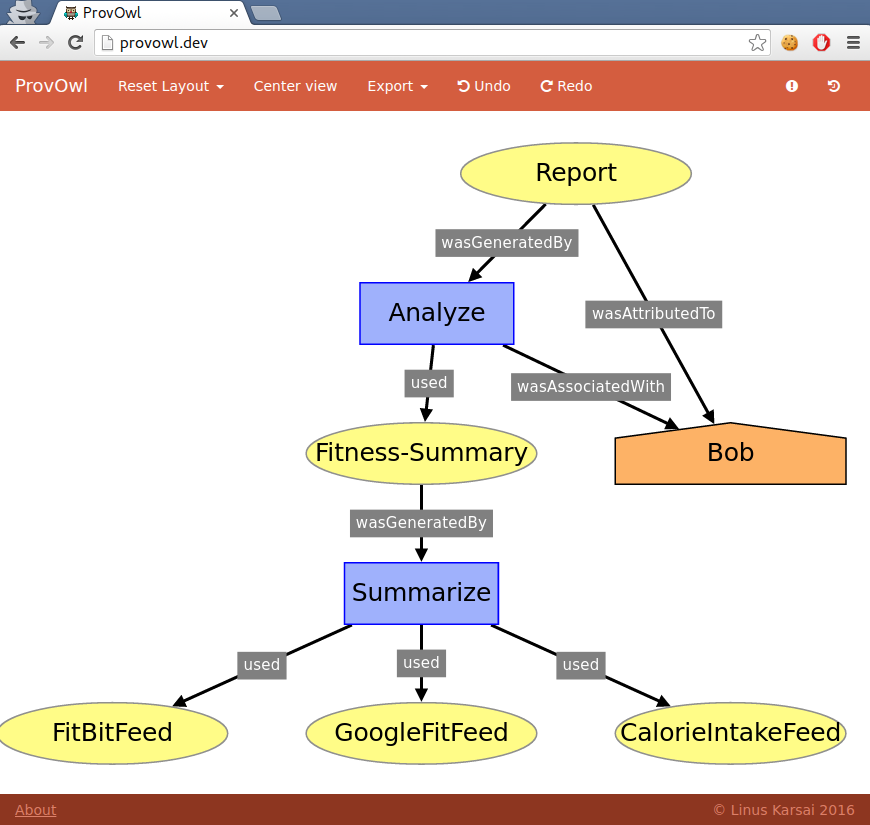
\includegraphics[width=\linewidth]{fitness-ungrouped}
	\caption{Provenance Data, as viewed in our \textit{ProvOwl} prototype. This labelled acyclic graph shows Bob's role in creating a report based on his fitness data. }
	\label{fig:fitness-ungrouped}
\end{figure}

\begin{figure}[h]
	\centering
	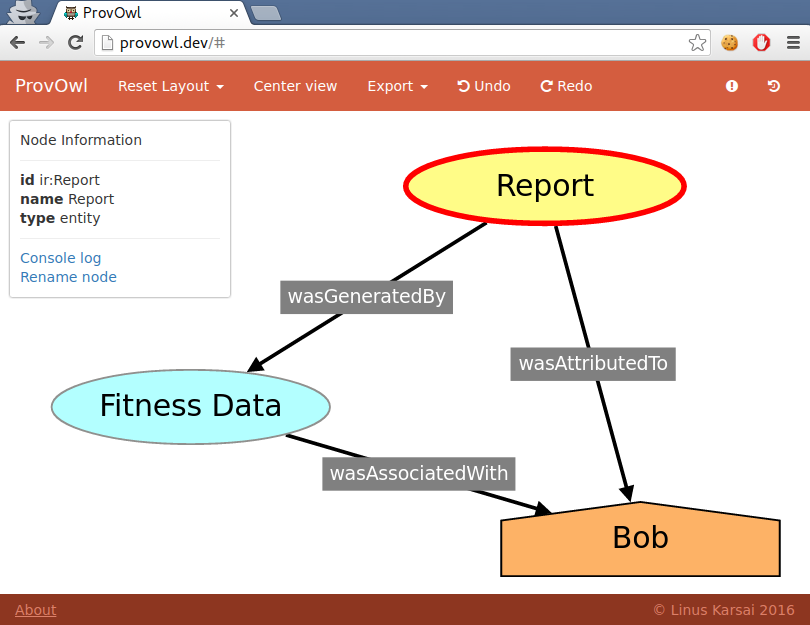
\includegraphics[width=\linewidth]{fitness-grouped}
	\caption{The graph of Fig.~\ref{fig:fitness-ungrouped}, after the user selected the \texttt{Analyze} node, with all its children, and clustered them, as a new node named \texttt{Fitness Data}. The user has selected the \texttt{Report} node, indicated by the red outline, and its details appear at the top left. Contextual actions are show in blue text in the details panel: \emph{Console log} is a debugging tool for printing the selected node to the console and \emph{Rename node} allows the user to change the name of the node. If multiple nodes where selected there would also be an option to group nodes.}
	\label{fig:fitness-grouped}
\end{figure}

\chapter{Challenges}
% Some challendges of showing/controlling clustered PROV
% Automatic clustering. 
% Naming. 
% False connections.

This clustering seems promising to reduce the size, and so, the complexity, of the visible provenance graph 
%% I altered this as it sounds passive but if the user actually did the action, that is very active
in an interface.
Many challenges remain about the ways to make the clustering interface work well for users, 
so they can do clustering, and then to explore the graph. This section discusses challenges we have encountered.

\section{Specification of user-defined clusters}
\label{sub:introduction_to_clustering}

A clustering action takes a set of nodes and combines them. 
Our interface follows the established interface method to select multiple items,
hold down \textit{ctrl} then click each node, once multiple nodes are selected a contextual link will appear in the details panel (like the blue links in Fig.~\ref{fig:fitness-grouped}) allowing the user to group them. 
This works well for combining a small number of nodes. 
When the user wants to combine a larger number of nodes, 
it would be useful to add a regular language, 
so the user can define a property for all the nodes to be clustered.
For example, suppose each day's Fitbit data was a separate node.
The user may want to cluster them to a single node,
with an expression such as ``cluster all the nodes where the name is `Fitbit-*-*-Jan-2016'.'' 
The language should be able to refer to a variety of node attributes, such as Date, Source, Type, etc.

This may go beyond just features of the node, to include the relationship between this node and others: 
for example, ``cluster all Fitbit nodes that are not used in a particular report.'' 
It may be useful to support parameterised clustering, 
where one command creates multiple clusters 
(for example, ``cluster all the Fitbit nodes from each month, separately, into a month-granularity cluster'). 
It will be challenging to design such a language, so that it is both powerful and easy to learn and use.
%
Some automation may help, with where the platform suggesting clusterings, based on workloads of provenance queries recorded (for example, one might cluster nodes which are frequently accessed together).

\section{Useful naming}

Once nodes have been clustered, it is difficult to automatically generate a name 
that the user will find meaningful for the new cluster~\cite{Schaffer1996, Abello2006}. 
Automating this process requires domain knowledge and it may also need deep models of the user and their needs.
This would be a substantial undertaking. 
For example, it may demand recognition that \textit{vim}, \textit{emacs} and \textit{nano} are all text editors? 
In an early version of our prototype, a new cluster-node was given a short random alpha-numeric name. 
However, this made the graph incomprehensible, with users needing to manually update the name immediately
so that they could understand the graph. 
Our current, still simple approach uses the name of the node in the cluster with the shortest distance from the root with the text ``group'' appended to the end. 
So, for example, in the transition from Figure~\ref{fig:fitness-ungrouped} to Figure~\ref{fig:fitness-grouped}, the node created would be named \textit{Fitness-Summary group}.


\section{Avoiding false dependencies}

Clustering is a simple type of graph rewriting, which creates an abstraction of the graph and in turn simplifies details of the original graph. This can produce false dependencies: these are newly implied lines of lineage, created by the clustering, and they falsely suggest that one entity had influence upon another. 
Worse yet, circular dependencies may occur, along with other violations of the constraints defined in the PROV-CONSTRAINT W3C document~\cite{w3c-prov-constraints}. For example, if the clustering set in the example of Fig.~\ref{fig:fitness-ungrouped} only included nodes \{\texttt{fitness-summary}, \texttt{CalorieIntakeFeed}\},  then a simple replacement of these nodes with a node $x$ would result in a circular dependency, namely $\langle x \; \mathtt{wasGeneratedBy} \; \mathtt{summarize}\rangle$ and $\langle \texttt{summarize} \; \texttt{used} \; x \rangle$, you can see this in Fig.~\ref{fig:loop}.
A theoretical formulation of provenance abstraction by \textit{grouping} (clustering) has been proposed in~\cite{Missier2014} to describe this and other problems that occur with clustering, along with simple algorithms for grouping arbitrary sets of nodes. 
Essentially, that work showed that to avoid false dependencies, as well as circular data dependencies, one must first compute a \textit{closure} operation that extends the user-selected nodes with all other nodes that sit on any path amongst these initial clustering nodes.
Combining this prior work with our user-oriented provenance navigation model can lead to a provably correct clustering mechanism. 
%A check could be made comparing suggested lineage of nodes around a cluster selecteion before and after a clustered node is created to see if any false connections exits. In some cases false connections may be desireable to obviscate sensitive information.

\begin{figure}[h]
	\centering
	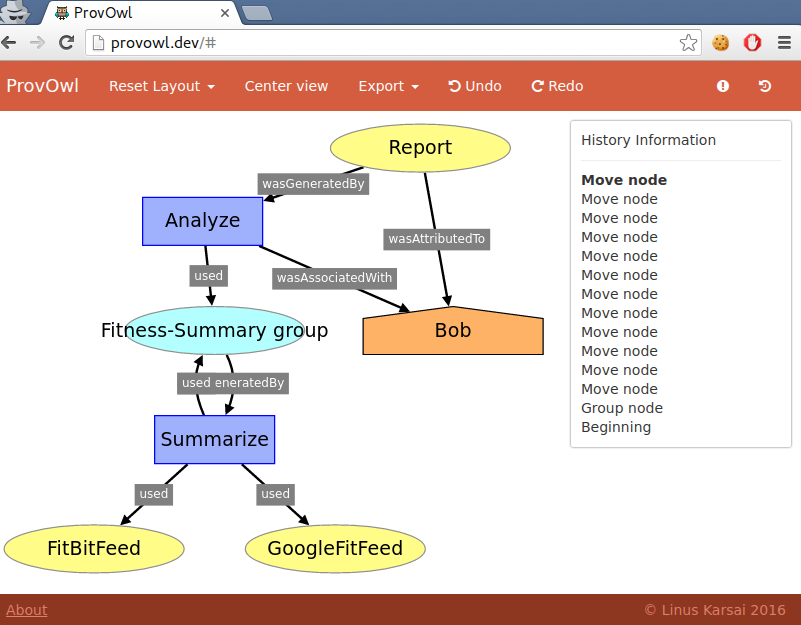
\includegraphics[width=\linewidth]{loop}
	\caption{When grouping on \{\texttt{fitness-summary}, \texttt{CalorieIntakeFeed}\} a circular dependency is caused between \texttt{Fitness-Summary group} and \texttt{Summarize}. The panel on the right can be toggled by the history button above and shows a list of user actions with the current state indicated in bold. Users can use the \textit{Undo} and \textit{Redo} buttons to move between actions.}
	\label{fig:loop}
\end{figure}


\chapter{Initial interface}
% Initial interface ideas, with a couple of screenshots, and a paragraph about implementation

Our interface reads provenance data stored in the PROV format~\cite{primer2013} and renders a directed acyclic graph that users can explore by zooming, panning, rearranging nodes and grouping nodes manually. 

%% IN UI work, accessible has special meaning
We implemented this as a web application. We use the Cytoscape.js\footnote{Cytoscape.js: Graph theory library for analysis and visualisation \url{http://js.cytoscape.org/}} because it has good support for graph theory. 
Files are loaded completely client-side, to reduce bandwidth. If faster analysis were required, it may require use of a combination of server-side and client-side processing.

%We implemented this interface as a web application because we had the highest level of expertise in web debelopment and it is a platform that is easily accessible by users. The standard technology for data visualisation in a browser is the D3.js\footnote{D3: Data Driven Documents \url{https://d3js.org/}} JavaScript library, however this interface is implemented using the Cytoscape.js\footnote{Cytoscape.js: Graph theory library for analysis and visualisation \url{http://js.cytoscape.org/}} because it specifically focuses on graph theory. Files are loaded completely client side in order to reduce bandwidth. If high powered analysis of provenance was required it may later be necessary to have server side processing in conjunction to client side processing. 

\section{Features}

This section explains how the design of our interface fulfils the seven visualisation tasks outlined by Ben Shneiderman~\cite{Shneiderman1996}: \textit{overview}, \textit{zoom}, \textit{filter}, \textit{details-on-demand}, \textit{relate}, \textit{history}, \textit{extract}. 

\subsection{Movement and Rearranging}
On first opening a provenance graph, the viewport is positioned to fit the entire graph on screen. This gives users an overview of the provenance. Users can then move the viewport around by clicking and dragging. Zooming is accomplished by using the scroll wheel. 

By default the graph's overall layout is determined using the JavaScript library dagre\footnote{Dagre: supports lay out of directed graphs client-side. The main skeleton of algorithm comes from ``A Technique for Drawing Directed Graphs''~\cite{Gansner1993}}, with other layout options, such as circle and breadth-first, available using the ``Reset Layout'' menu (visible on the top bar, second from the left in the figures). Users can also re-arrange nodes as they wish by clicking and dragging on a node. 

\subsection{Details-on-demand}
Selecting a node shows the details panel, as in Fig.~\ref{fig:fitness-grouped}. This displays other information about the node and contextual functions such as renaming nodes (the blue link at the bottom of the panel) or grouping nodes.

\subsection{Grouping}

Users can select multiple nodes at once, by clicking on each whilst holding down \textit{ctrl}. 
Once multiple nodes have been selected, the information panel will contain a link to group the nodes. 
Selecting this moves the nodes together, replacing them with a single composite node, represented by a light blue oval, 
with default name based on the name of the node closest to the root plus the word ``group''. 

\subsection{History}

%A vital task in exploration interfaces is that of history~\cite{Shneiderman1996}. 
Having the ability to undo and redo 
actions is critical to ensure that users can confidently and safely explore the information, 
without fear of causing permanent damage~\cite{Shneiderman1996}. 
Our interface tracks the movement and grouping of nodes. 
Then undo and redo buttons allow users to step through through these actions. 
A history pane can be toggled, by clicking the top right history icon (this pane is visible on the right of Fig.~\ref{fig:loop}), to show what current step of history a user is at.

\subsection{Sharing}

The ``Export'' menu item (in the top bar of the figures)
saves an image of the current graph with all the user modifications. 
This can either save the entire graph or be limited to the current viewport,
if the user wanted to focus on a certain section.

\chapter{Future Work}
The prototype source code is available on GitHub\footnote{\url{https://github.com/karsai5/ProvOwl}}. The interface is also available online where you can test it with a sample graph\footnote{\url{http://provowl.com/?file=/prov-examples/provn/threenode.provn}}.
We describe features under development to improve usability.

We propose to create a regular expression language to select nodes, as mentioned in the section on challenges. 
This will enable users to select nodes in cases such as:
(i) Select all nodes with the name ``*Feed''
(ii) Select all nodes \textit{not} influencing the ``Summarize'' node
(iii) Select all children of ``Fitness-Summary''.
For large graphs, this could allow for faster user-directed simplification of a graph. 

As an extension of this, the language should describe parametered clustering, so users ask for multiple similar clusters to be formed. For example ``Create clusters from nodes the same depth from the root'' or even using data inside the nodes ``Create clusters from nodes that have the same creation date''.  

This could also impact the way nodes are automatically named. If the user created clusters from nodes that all have the same creation date, the system may infer that the name for the new node should include the creation date.

We also wish to extend the PROV standard to include descriptions of cluster nodes. This would allow a user to cluster nodes manually, export the PROV file with cluster descriptions and then share with someone else. This \textit{extraction}, being able to export your current state of exploration, would allow further exploration from the current state later on or even sharing with other users for further analysis.


%\balancecolumns % GM June 2007
% That's all folks!
% \bibliography{bibliography,bibliography_PM}
% \bibliographystyle{myplain}
% \end{document}
